% Created 2020-11-10 mar 16:06
% Intended LaTeX compiler: pdflatex
\documentclass[11pt]{article}
\usepackage[utf8]{inputenc}
\usepackage[T1]{fontenc}
\usepackage{graphicx}
\usepackage{grffile}
\usepackage{longtable}
\usepackage{wrapfig}
\usepackage{rotating}
\usepackage[normalem]{ulem}
\usepackage{amsmath}
\usepackage{textcomp}
\usepackage{amssymb}
\usepackage{capt-of}
\usepackage{hyperref}
\author{Claudio Vaucheret}
\date{\textit{<2018-10-23 mar>}}
\title{Conceptos Avanzados en Lenguajes de Programación}
\hypersetup{
 pdfauthor={Claudio Vaucheret},
 pdftitle={Conceptos Avanzados en Lenguajes de Programación},
 pdfkeywords={},
 pdfsubject={},
 pdfcreator={Emacs 26.1 (Org mode 9.1.14)}, 
 pdflang={English}}
\begin{document}

\maketitle

\section*{Introducción}
\label{sec:orgb1faf2d}
\subsection*{Tiempo de Vida del Objeto y Ligadura}
\label{sec:org8caa5d2}

\begin{itemize}
\item Creación del objeto
\item Creación de las ligaduras
\item Referencias a variables, subrutinas, tipos, todos los cuales usan
las ligaduras
\item Desactivación y reactivación de ligaduras que pueden estar
temporariamente en desuso
\item Destrucción de ligaduras
\item Destrucción de los objetos
\end{itemize}

\subsection*{Tiempos de vida distintos}
\label{sec:orge912182}
\begin{itemize}
\item Referencias colgadas
\begin{itemize}
\item La ligadura sobrevive al objeto
\end{itemize}
\item Almacenamiento sin referencias (basura)
\begin{itemize}
\item El objeto sobrevive a su ligadura
\end{itemize}
\end{itemize}


\subsection*{Mecanismos de alojamiento}
\label{sec:org89151a4}
\begin{itemize}
\item Estático
\begin{itemize}
\item A los objetos se les da una dirección absoluta que es retenida a
través de la ejecución del programa
\end{itemize}
\item Basado en Pila
\begin{itemize}
\item Los objetos son alojados y desalojados en un orden LIFO
\end{itemize}
\item \emph{Heap}
\begin{itemize}
\item Los objetos pueden ser ser alojados y desalojados en momentos
arbitrarios. Requiere algoritmos de administración mas generales y caros.
\end{itemize}
\end{itemize}

\subsection*{Alojamiento Estático}
\label{sec:orgfb9366c}
\begin{itemize}
\item Código
\item Variables Globales
\item variables \emph{static} u \emph{own}
\item constantes explícitas
\item tablas de soporte en tiempo de ejecución
\end{itemize}

\subsubsection*{Subrutinas}
\label{sec:orgace0ed5}
\begin{center}
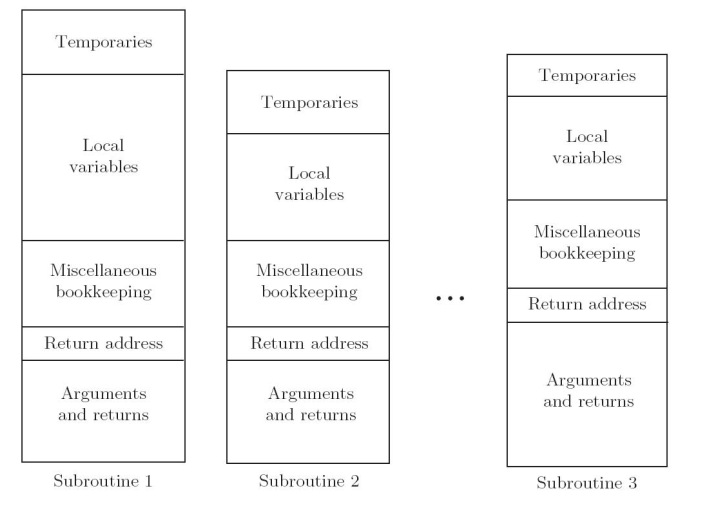
\includegraphics[width=.9\linewidth]{aljamestaticosub.png}
\end{center}

\subsection*{Alojamiento basado en Pila}
\label{sec:orgcf08940}

\begin{itemize}
\item Pila central para:
\begin{itemize}
\item parámetros
\item variables locales
\item datos temporales
\end{itemize}
\item Porqué una Pila?
\begin{itemize}
\item aloja espacio para rutinas recursivas (no necesario en FORTRAN sin recursión)
\item reuso del espacio (En todos los lenguajes)
\end{itemize}
\end{itemize}

\subsubsection*{Subrutinas}
\label{sec:orgcf4e82d}

\begin{center}
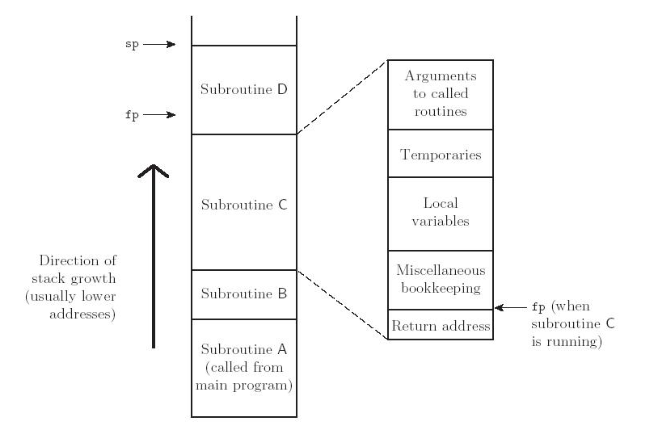
\includegraphics[width=.9\linewidth]{alojpilasubr.png}
\end{center}

\subsubsection*{Alojamiento basado en Pila}
\label{sec:orge62f548}
\begin{itemize}
\item Contenido de un Registro de Activación
\begin{itemize}
\item Argumentos y Resultado
\item variables locales
\item Datos temporales
\item Datos de mantenimiento (registros guardados, número de lineas
estático, links etc)
\end{itemize}
\item A las variables locales y Argumentos se les asigna un desplazamiento
FIJO (a partir del puntero de pila o puntero de registro de
activación) en tiempo de compilación.
\end{itemize}

\subsubsection*{Alojamiento basado en Pila}
\label{sec:org7bef60c}
\begin{itemize}
\item El mantenimiento de la Pila es responsabilidad de la \emph{secuencia de
llamado} del llamador, y de el \emph{prologo} y el \emph{epilogo} de la
subrutina llamada.
\begin{itemize}
\item se ahorra espacio colocando todo lo posible en el \emph{prologo} y en
el \emph{epilogo}
\item se puede ahorrar tiempo
\begin{itemize}
\item colocando material en el llamador  o
\item combinado lo que es conocido en ambos lugares (optimización interprocedural)
\end{itemize}
\end{itemize}
\end{itemize}

\section*{Alojamiento basado en \emph{Heap}}
\label{sec:org6e8af8f}
\begin{itemize}
\item Alojamiento Dinámico
\end{itemize}

\begin{center}
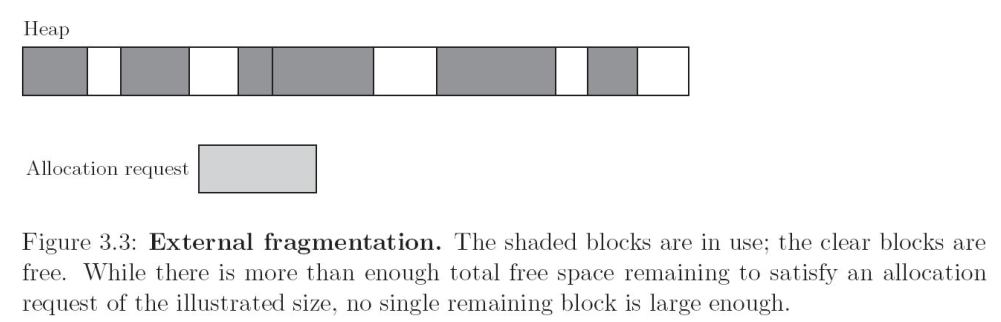
\includegraphics[width=.9\linewidth]{alojdinheap.png}
\end{center}

\subsubsection*{Alojamiento basado en \emph{Heap}}
\label{sec:orgc762b44}
\begin{itemize}
\item Muchas posibles estrategias
\item compromiso entre espacio y tiempo
\item Fragmentación
\begin{itemize}
\item interna (se aloja un bloque que es mas grande que el requerido
para el objeto)
\item externa (cuando los bloques asignados para los objetos de datos
estan distribuidos en todo el heap de tal modo que el espacio
restante esta compuesto de muchos bloques muy pequeños. Hay
suficiente espacio pero ninguna pieza suficientemente grande para
alojar un nuevo requerimiento.
\end{itemize}
\end{itemize}

\subsubsection*{Alojamiento basado en \emph{Heap}}
\label{sec:org1a56da3}
\begin{itemize}
\item Lista ligado de bloques libres
\item Algoritmos de asignación
\begin{itemize}
\item \emph{First fit} selecciona el primer bloque de la lista que es
suficientemente grande para satisfacer el requerimiento.
\item \emph{Best fit} busca la lista entera para encontrar el bloque mas
chico suficientemente grande para alojar el objeto
\end{itemize}
\item Varias listas libres separadas por tamaño. La división puede ser
estática o dinámica
\begin{itemize}
\item \emph{Buddy System} 
\begin{itemize}
\item potencia de 2. si un bloque de \(2^k\) se necesita y ninguno es
diponible se divide uno de \(2^{k+1}\)
\end{itemize}
\item \emph{Fibonacci heap}
\begin{itemize}
\item numeros de fibonacci para los tamaños estandars
\end{itemize}
\end{itemize}
\end{itemize}


\subsubsection*{Alojamiento basado en \emph{Heap}}
\label{sec:org243a95b}
\begin{itemize}
\item El problema de referencias sueltas (dangling) son debidas a
\begin{itemize}
\item desalojo explícito de objetos del \emph{heap}
\begin{itemize}
\item solo en lenguajes con desalojo explícito
\end{itemize}
\item desalojo implícito de objetos elaborados
\end{itemize}
\item Dos mecanismos de implementación para manejar referencias sueltas:
\begin{itemize}
\item Lápidas (\emph{Tombestones})
\item Llaves y cerrojos (\emph{Locks and Keys})
\end{itemize}
\end{itemize}

\subsubsection*{Alojamiento basado en \emph{Heap}}
\label{sec:org75cb0d7}
\begin{itemize}
\item \emph{Tombstones}
\end{itemize}
\begin{center}
\begin{center}
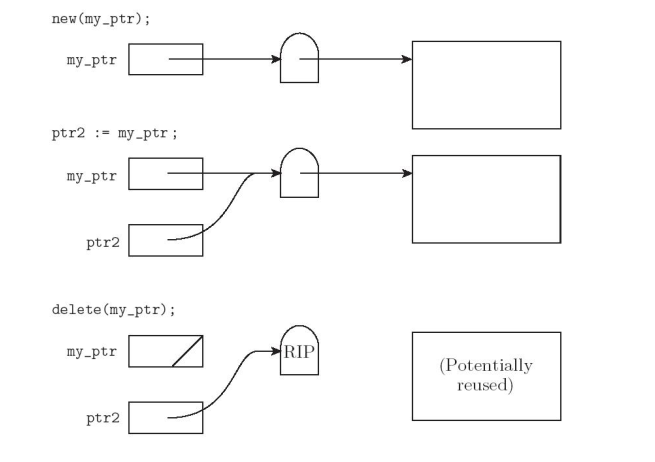
\includegraphics[width=.9\linewidth]{tombstones.png}
\end{center}
\end{center}
\subsubsection*{Alojamiento basado en \emph{Heap}}
\label{sec:org4a02ce7}
\begin{itemize}
\item \emph{Locks and Keys}
\end{itemize}
\begin{center}
\begin{center}
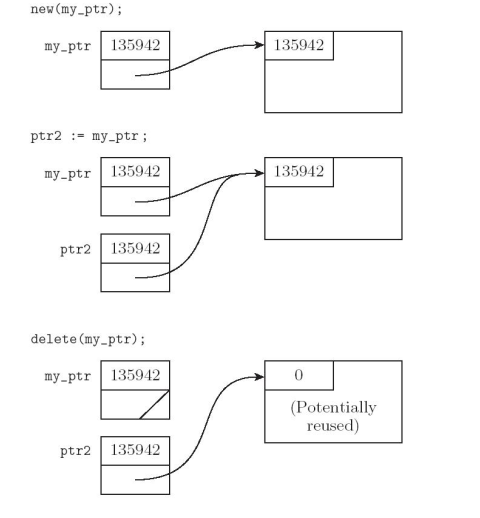
\includegraphics[width=.9\linewidth]{lockskeys.png}
\end{center}
\end{center}

\subsubsection*{Recolección de Basura}
\label{sec:org1797c3c}
\begin{itemize}
\item \emph{garbage collection}
\begin{itemize}
\item esencial en lenguajes funcionales y lógicos
\item se volvió popular en lenguajes imperativos
\end{itemize}
\item Contador de referencias
\end{itemize}
\begin{center}
\begin{center}
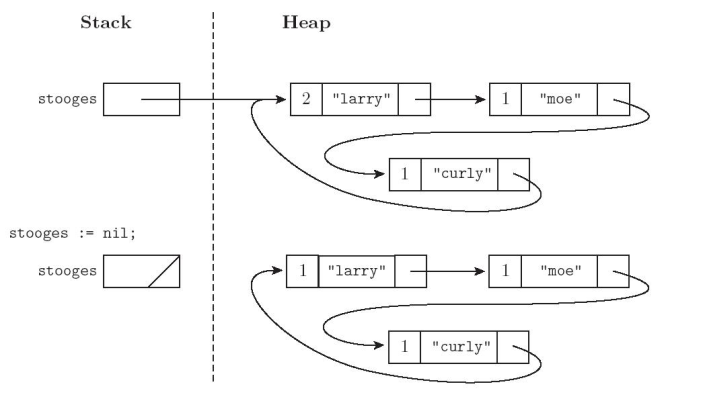
\includegraphics[width=.9\linewidth]{contadref.png}
\end{center}
\end{center}
\subsubsection*{Trazado de la colección}
\label{sec:org0a372b2}
\begin{itemize}
\item marcado y barrido (\emph{mark and Sweep}
\begin{enumerate}
\item El recolector camina a través del \emph{heap} marcando todo bloque como
"usable" tentativamente
\item Comenzando de punteros de afuera del \emph{heap}, recursivamente
explora todos las estructuras de datos ligadas, marcando cada
bloque nuevo descubierto como "usado"
\item El recolector recorre de nuevo el \emph{heap}, moviendo todo bloque
aún marcado como "usable" a la lista de bloques libres.
\end{enumerate}
\end{itemize}

\subsubsection*{Recolección de Basura}
\label{sec:org3d766b2}
\begin{itemize}
\item Reversión de puntero
\end{itemize}

\begin{center}
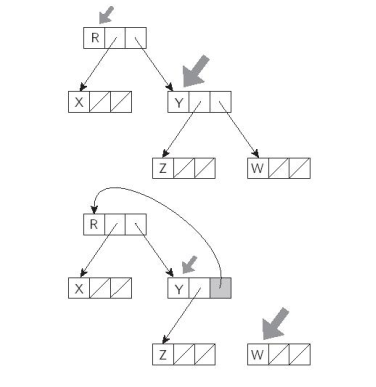
\includegraphics[width=.9\linewidth]{reversepoint.png}
\end{center} 

\subsubsection*{Recolección de Basura}
\label{sec:orga1f97be}
\begin{itemize}
\item Otras alternativas
\begin{itemize}
\item Parar y Copiar
\item Recolección Generacional
\item Recolección Conservadora
\end{itemize}
\end{itemize}
Emacs 26.1 (Org mode 9.1.14)
\end{document}